\documentclass[11pt,a4paper]{report}
\usepackage[textwidth=37em,vmargin=30mm]{geometry}
\usepackage{calc,xunicode,amsmath,amssymb,paralist,enumitem,tabu,booktabs,datetime2,xeCJK,xeCJKfntef,listings}
\usepackage{tocloft,fancyhdr,tcolorbox,xcolor,graphicx,eso-pic,xltxtra,xelatexemoji}

\newcommand{\envyear}[0]{2025}
\newcommand{\envdatestr}[0]{2025-04-09}
\newcommand{\envfinaldir}[0]{webdb/2025/20250409/final}

\usepackage[hidelinks]{hyperref}
\hypersetup{
    colorlinks=false,
    pdfpagemode=FullScreen,
    pdftitle={Web Digest - \envdatestr}
}

\setlength{\cftbeforechapskip}{10pt}
\renewcommand{\cftchapfont}{\rmfamily\bfseries\large\raggedright}
\setlength{\cftbeforesecskip}{2pt}
\renewcommand{\cftsecfont}{\sffamily\small\raggedright}

\setdefaultleftmargin{2em}{2em}{1em}{1em}{1em}{1em}

\usepackage{xeCJK,xeCJKfntef}
\xeCJKsetup{PunctStyle=plain,RubberPunctSkip=false,CJKglue=\strut\hskip 0pt plus 0.1em minus 0.05em,CJKecglue=\strut\hskip 0.22em plus 0.2em}
\XeTeXlinebreaklocale "zh"
\XeTeXlinebreakskip = 0pt


\setmainfont{Brygada 1918}
\setromanfont{Brygada 1918}
\setsansfont{IBM Plex Sans}
\setmonofont{JetBrains Mono NL}
\setCJKmainfont{Noto Serif CJK SC}
\setCJKromanfont{Noto Serif CJK SC}
\setCJKsansfont{Noto Sans CJK SC}
\setCJKmonofont{Noto Sans CJK SC}

\setlength{\parindent}{0pt}
\setlength{\parskip}{8pt}
\linespread{1.15}

\lstset{
	basicstyle=\ttfamily\footnotesize,
	numbersep=5pt,
	backgroundcolor=\color{black!5},
	showspaces=false,
	showstringspaces=false,
	showtabs=false,
	tabsize=2,
	captionpos=b,
	breaklines=true,
	breakatwhitespace=true,
	breakautoindent=true,
	linewidth=\textwidth
}






\newcommand{\coverpic}[2]{
    % argv: itemurl, authorname
    Cover photo by #2~~(\href{#1}{#1})
}
\newcommand{\makeheader}[0]{
    \begin{titlepage}
        % \newgeometry{hmargin=15mm,tmargin=21mm,bmargin=12mm}
        \begin{center}
            
            \rmfamily\scshape
            \fontspec{BaskervilleF}
            \fontspec{Old Standard}
            \fontsize{59pt}{70pt}\selectfont
            WEB\hfill DIGEST
            
            \vfill
            % \vskip 30pt
            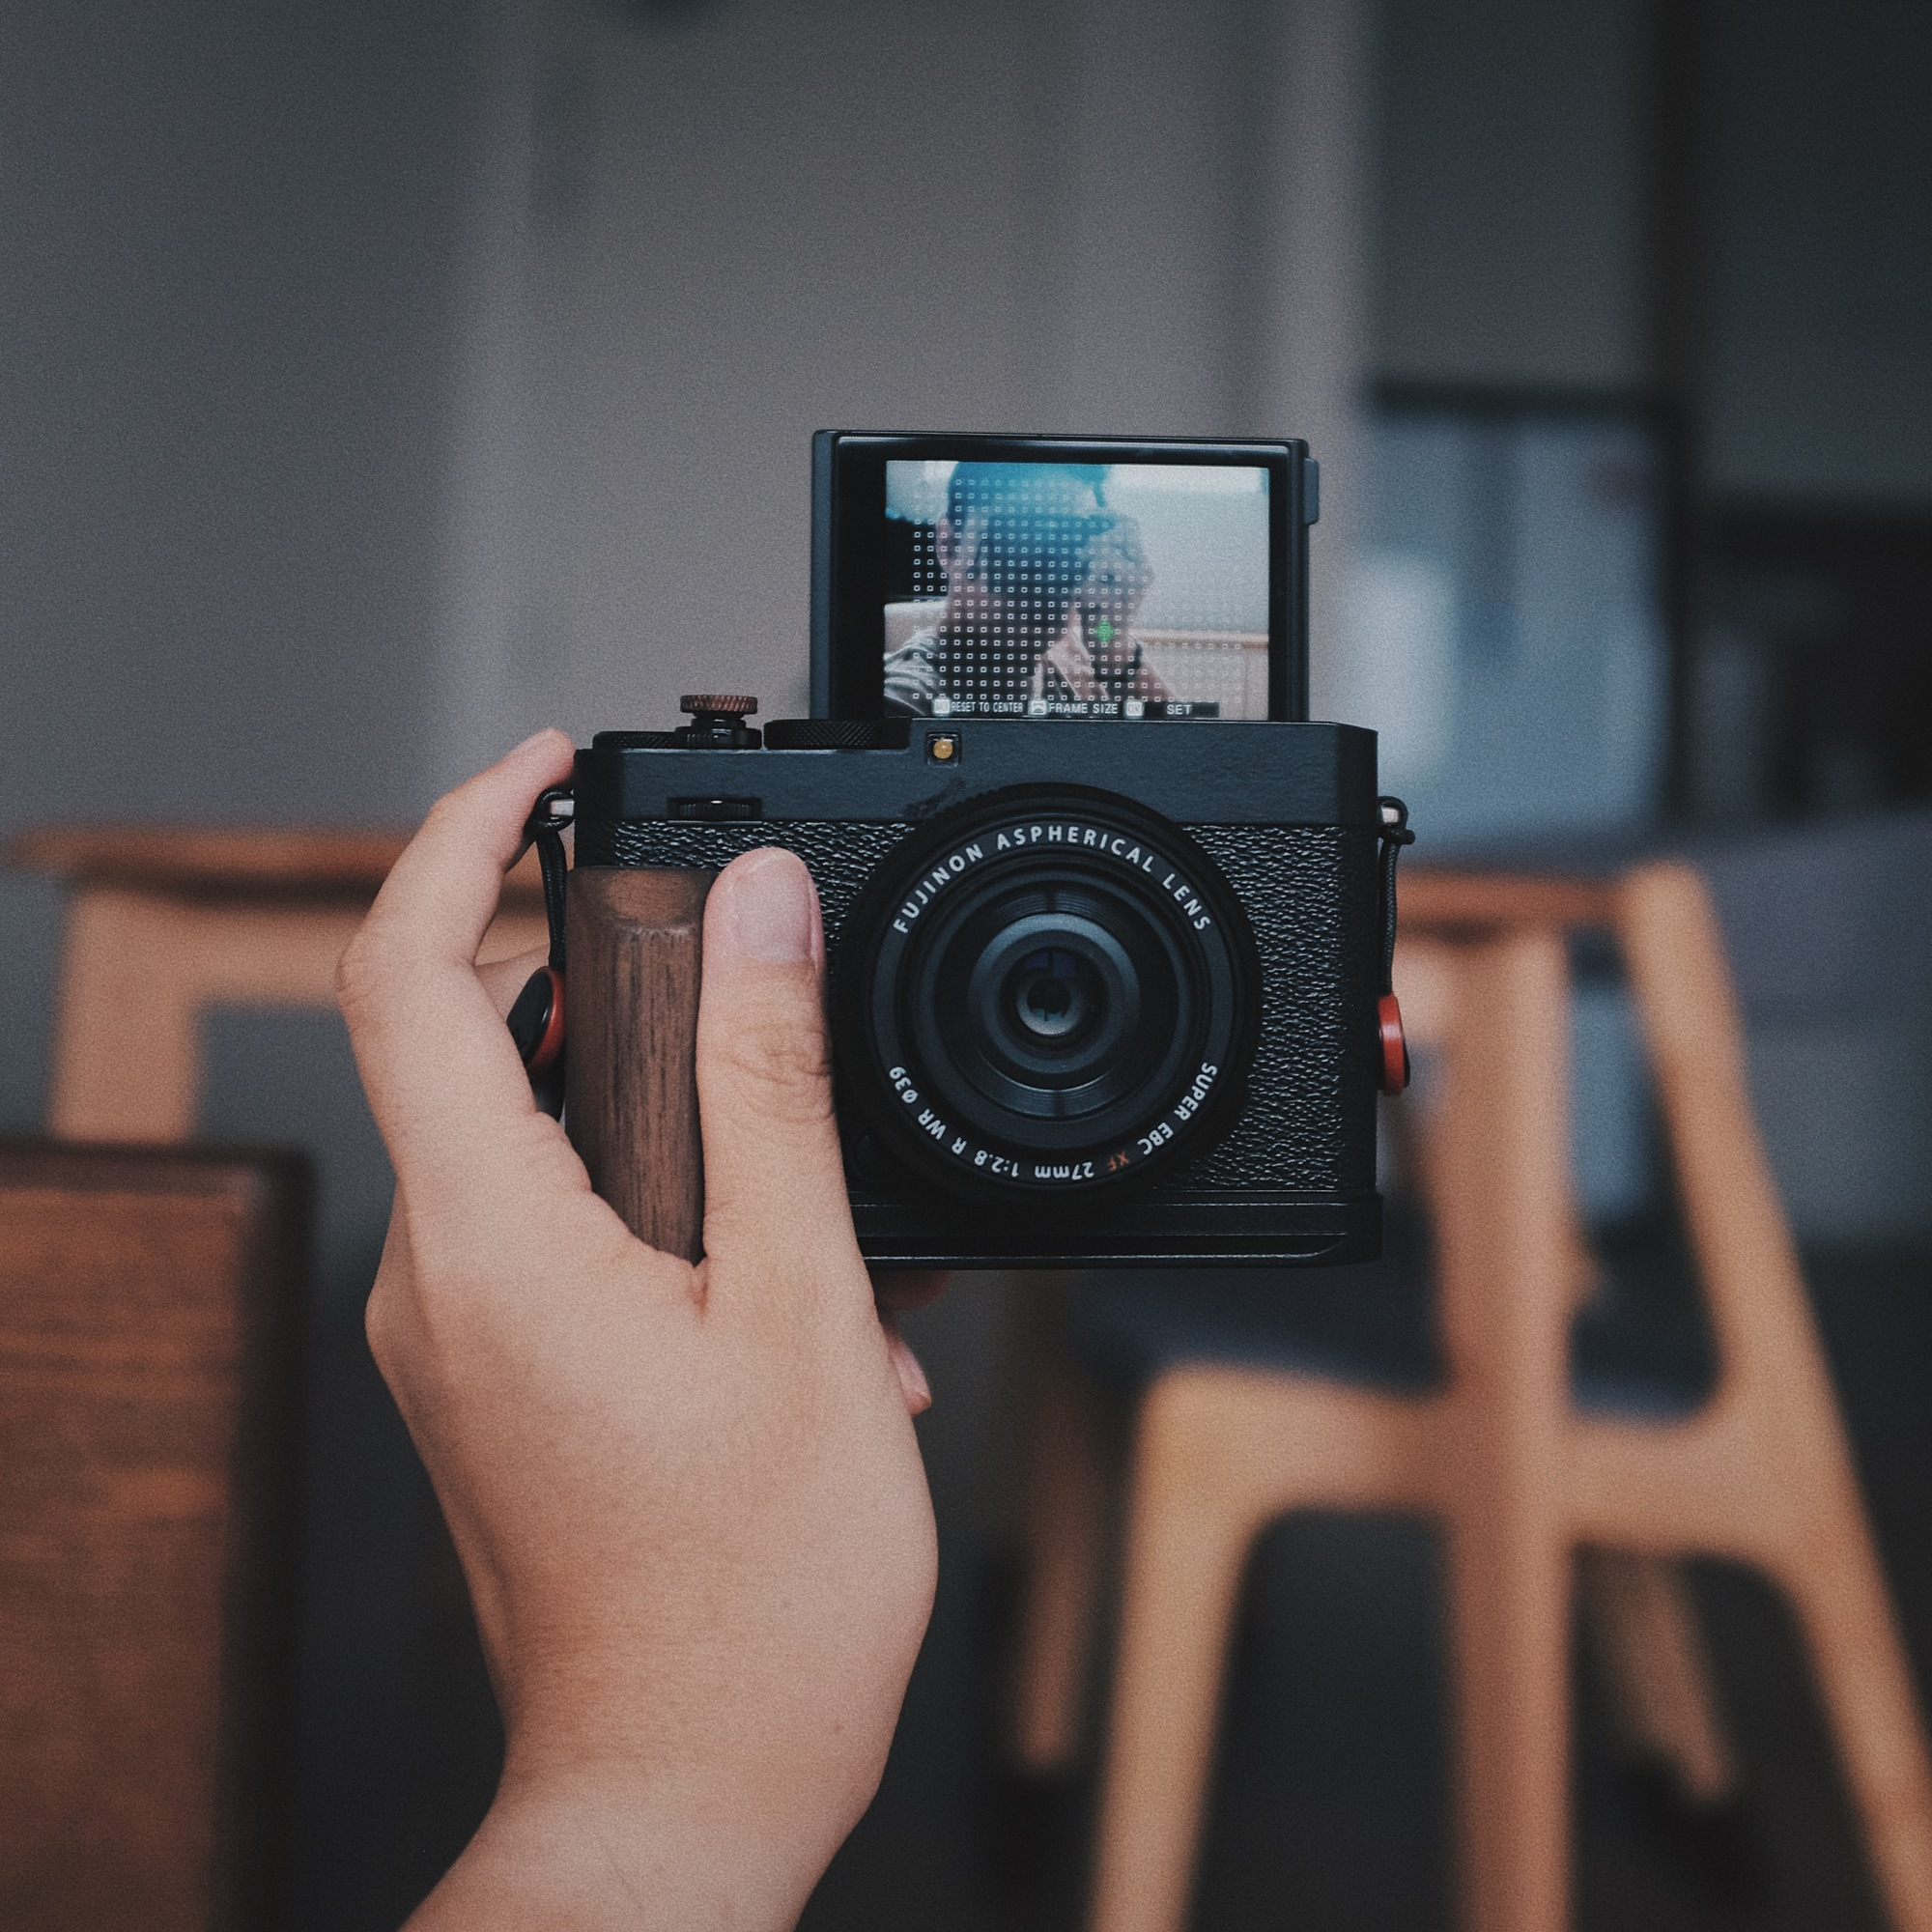
\includegraphics[width=\linewidth]{\envfinaldir/coverpic-prod.jpg}\par
            % \vskip 30pt
            \vfill

            \normalsize\rmfamily\scshape
            \copyright{} The Web Digest Project \hfill\large \envdatestr
        \end{center}
    \end{titlepage}
    % \restoregeometry
}
\newcommand{\simplehref}[1]{%
    \textcolor{blue!80!green}{\href{#1}{#1}}%
}
\renewcommand{\contentsname}{\center\Huge\sffamily\bfseries Contents\par\vskip 20pt}
\newcounter{ipartcounter}
\setcounter{ipartcounter}{0}
\newcommand{\ipart}[1]{
    % \vskip 20pt
    \clearpage
    \stepcounter{ipartcounter}
    \phantomsection
    \addcontentsline{toc}{chapter}{#1}
    % \begin{center}
    %     \Huge
    %     \sffamily\bfseries
    %     #1
    % \end{center}
    % \vskip 20pt plus 7pt
}
\newcounter{ichaptercounter}
\setcounter{ichaptercounter}{0}
\newcommand{\ichapter}[1]{
    % \vskip 20pt
    \clearpage
    \stepcounter{ichaptercounter}
    \phantomsection
    \addcontentsline{toc}{section}{\numberline{\arabic{ichaptercounter}}#1}
    \begin{center}
        \Huge
        \sffamily\bfseries
        #1
    \end{center}
    \vskip 20pt plus 7pt
}
\newcommand{\entrytitlefont}[1]{\subsection*{\raggedright\Large\sffamily\bfseries#1}}
\newcommand{\entryitemGeneric}[2]{
    % argv: title, url
    \parbox{\linewidth}{
        \entrytitlefont{#1}\par\vskip 5pt
        \footnotesize\ttfamily\mdseries
        \simplehref{#2}
    }\vskip 11pt plus 11pt minus 1pt
}
\newcommand{\entryitemGithub}[3]{
    % argv: title, url, desc
    \parbox{\linewidth}{
        \entrytitlefont{#1}\par\vskip 5pt
        \footnotesize\ttfamily\mdseries
        \simplehref{#2}\par\vskip 5pt
        \small\rmfamily\mdseries#3
    }\vskip 11pt plus 11pt minus 1pt
}
\newcommand{\entryitemAp}[3]{
    % argv: title, url, desc
    \parbox{\linewidth}{
        \entrytitlefont{#1}\par\vskip 5pt
        \footnotesize\ttfamily\mdseries
        \simplehref{#2}\par\vskip 5pt
        \small\rmfamily\mdseries#3
    }\vskip 11pt plus 11pt minus 1pt
}
\newcommand{\entryitemHackernews}[3]{
    % argv: title, hnurl, rawurl
    % \parbox{\linewidth}{
    %     \entrytitlefont{#1}\par\vskip 5pt
    %     \footnotesize\ttfamily\mdseries
    %     \simplehref{#3}\par
    %     \textcolor{black!50}{\href{#2}{#2}}
    % }\vskip 11pt plus 11pt minus 1pt
    \begin{minipage}{\linewidth}
            \entrytitlefont{#1}\par\vskip 5pt
            \footnotesize\ttfamily\mdseries
            \simplehref{#3}\par
            \textcolor{black!50}{\href{#2}{#2}}
    \end{minipage}\par\vskip 11pt plus 11pt minus 1pt
}







\begin{document}

\makeheader

\tableofcontents\clearpage




\ipart{Developers}
\ichapter{Hacker News}
\entryitemTwoLinks{Obituary for Cyc}{https://news.ycombinator.com/item?id=43625474}{https://yuxi-liu-wired.github.io/essays/posts/cyc/}

\entryitemTwoLinks{Apache ECharts}{https://news.ycombinator.com/item?id=43624220}{https://echarts.apache.org/en/index.html}

\entryitemTwoLinks{Thank HN: The puzzle game I posted here 6 weeks ago got licensed by The Atlantic}{https://news.ycombinator.com/item?id=43622719}{https://www.theatlantic.com/games/bracket-city/}

\entryitemTwoLinks{Better typography with text-wrap pretty}{https://news.ycombinator.com/item?id=43622703}{https://webkit.org/blog/16547/better-typography-with-text-wrap-pretty/}

\entryitemTwoLinks{Show HN: Connecting an IBM 3151 terminal to a mainframe [video]}{https://news.ycombinator.com/item?id=43621007}{https://www.youtube.com/watch?v=V14ac9cRi9Q}

\entryitemTwoLinks{Meta got caught gaming AI benchmarks}{https://news.ycombinator.com/item?id=43620452}{https://www.theverge.com/meta/645012/meta-llama-4-maverick-benchmarks-gaming}

\entryitemTwoLinks{Brazil's government-run payments system has become dominant}{https://news.ycombinator.com/item?id=43620279}{https://www.economist.com/the-americas/2025/04/03/brazils-government-run-payments-system-has-become-dominant}

\entryitemTwoLinks{Tailscale has raised \$160M}{https://news.ycombinator.com/item?id=43620141}{https://tailscale.com/blog/series-c}

\entryitemTwoLinks{'Unstoppable force' of solar power propels world to 40\% clean electricity}{https://news.ycombinator.com/item?id=43620007}{https://news.sky.com/story/unstoppable-force-of-solar-power-propels-world-to-40-clean-electricity-report-finds-13344230}

\entryitemTwoLinks{Ask HN: Do you still use search engines?}{https://news.ycombinator.com/item?id=43619768}{https://news.ycombinator.com/item?id=43619768}

\entryitemTwoLinks{An Overwhelmingly Negative and Demoralizing Force}{https://news.ycombinator.com/item?id=43619759}{https://aftermath.site/ai-video-game-development-art-vibe-coding-midjourney}

\entryitemTwoLinks{Less Htmx Is More}{https://news.ycombinator.com/item?id=43619581}{https://unplannedobsolescence.com/blog/less-htmx-is-more/}

\entryitemTwoLinks{Intelligence Evolved at Least Twice in Vertebrate Animals}{https://news.ycombinator.com/item?id=43619548}{https://www.quantamagazine.org/intelligence-evolved-at-least-twice-in-vertebrate-animals-20250407/}

\entryitemTwoLinks{UK Effort to Keep Apple Encryption Fight Secret Is Blocked}{https://news.ycombinator.com/item?id=43619315}{https://www.msn.com/en-us/money/other/uk-effort-to-keep-apple-encryption-fight-secret-is-blocked/ar-AA1CsokD}

\entryitemTwoLinks{Building the System/360 Mainframe Nearly Destroyed IBM}{https://news.ycombinator.com/item?id=43619229}{https://spectrum.ieee.org/building-the-system360-mainframe-nearly-destroyed-ibm}

\entryitemTwoLinks{India's repair culture gives new life to dead laptops}{https://news.ycombinator.com/item?id=43618105}{https://www.theverge.com/tech/639126/india-frankenstein-laptops}

\entryitemTwoLinks{Any program can be a GitHub Actions shell}{https://news.ycombinator.com/item?id=43617493}{https://yossarian.net/til/post/any-program-can-be-a-github-actions-shell/}

\entryitemTwoLinks{North Korean IT workers have infiltrated the Fortune 500}{https://news.ycombinator.com/item?id=43617352}{https://www.yahoo.com/news/thousands-north-korean-workers-infiltrated-110000417.html}

\entryitemTwoLinks{Framework temporarily pausing some laptop sales in the US due to tariffs}{https://news.ycombinator.com/item?id=43617207}{https://fosstodon.org/@frameworkcomputer/114297967333461078}

\entryitemTwoLinks{What Was Quartz?}{https://news.ycombinator.com/item?id=43616604}{https://www.zachseward.com/what-was-quartz/}\ichapter{Phoronix}
\entryitemGeneric{\hskip 0pt{}PostgreSQL Merges Initial Support For NUMA Awareness}{https://www.phoronix.com/news/PostgreSQL-Lands-NUMA-Awareness}

\entryitemGeneric{\hskip 0pt{}UALink 200G 1.0 Specification Published For Connecting Up To 1,024 Accelerators}{https://www.phoronix.com/news/UALink-200G-1.0-Released}

\entryitemGeneric{\hskip 0pt{}Linux 6.15 Features Deliver A Lot For Intel \& AMD, Many Other Changes}{https://www.phoronix.com/review/linux-615-features}

\entryitemGeneric{\hskip 0pt{}Blender Is Looking For Help Testing Its Maturing Vulkan Backend}{https://www.phoronix.com/news/Blender-Vulkan-Help-Testing}

\entryitemGeneric{\hskip 0pt{}OpenSSL 3.5 LTS Released With Server-Side QUIC}{https://www.phoronix.com/news/OpenSSL-3.5-Released}

\entryitemGeneric{\hskip 0pt{}Wayland Protocols 1.43 Released With Toplevel Tag Protocol}{https://www.phoronix.com/news/Wayland-Protocols-1.43}

\entryitemGeneric{\hskip 0pt{}CUPS 2.4.12 Released To End Out The CUPS 2.4 Print Server Series}{https://www.phoronix.com/news/CUPS-2.4.12-Released}

\entryitemGeneric{\hskip 0pt{}Linux Patches Revised For The Lenovo Gaming Series WMI Drivers}{https://www.phoronix.com/news/Lenovo-Gaming-Series-WMI-v5}

\entryitemGeneric{\hskip 0pt{}Ubuntu Adds Support For A New Low-Cost RISC-V Board: The OrangePi RV2 8GB For ~\$64}{https://www.phoronix.com/news/Ubuntu-Linux-On-OrangePi-RV2}\ichapter{Dribbble}
\entryitemGeneric{\hskip 0pt{}Nite Riot®\_Film Production // Case Study\_Vol.1.0}{https://dribbble.com/shots/25874978-Nite-Riot-Film-Production-Case-Study-Vol-1-0}

\entryitemGeneric{\hskip 0pt{}Howzit}{https://dribbble.com/shots/25871668-Howzit}

\entryitemGeneric{\hskip 0pt{}Brainstorm}{https://dribbble.com/shots/25871145-Brainstorm}

\entryitemGeneric{\hskip 0pt{}Boxplates}{https://dribbble.com/shots/25869902-Boxplates}

\entryitemGeneric{\hskip 0pt{}Crypto Mobile App}{https://dribbble.com/shots/25869253-Crypto-Mobile-App}

\entryitemGeneric{\hskip 0pt{}Spark illustrations}{https://dribbble.com/shots/25872229-Spark-illustrations}

\entryitemGeneric{\hskip 0pt{}Educational Website on Space Pollution}{https://dribbble.com/shots/25860515-Educational-Website-on-Space-Pollution}

\entryitemGeneric{\hskip 0pt{}Going for Gold}{https://dribbble.com/shots/25861716-Going-for-Gold}

\entryitemGeneric{\hskip 0pt{}LA Kings Mexican Heritage Theme Night Art}{https://dribbble.com/shots/25862720-LA-Kings-Mexican-Heritage-Theme-Night-Art}

\entryitemGeneric{\hskip 0pt{}CRYSTAL PRT\_2 // Mobile Version}{https://dribbble.com/shots/25860264-CRYSTAL-PRT-2-Mobile-Version}

\entryitemGeneric{\hskip 0pt{}Atomiq Unused Logo Design}{https://dribbble.com/shots/25861903-Atomiq-Unused-Logo-Design}

\entryitemGeneric{\hskip 0pt{}Hexagon + Waves Abstract Logo Concept}{https://dribbble.com/shots/25860795-Hexagon-Waves-Abstract-Logo-Concept}

\entryitemGeneric{\hskip 0pt{}Downlink}{https://dribbble.com/shots/25860034-Downlink}

\entryitemGeneric{\hskip 0pt{}Ship Logo Design - Boat, Shield, Star, Waves}{https://dribbble.com/shots/25854151-Ship-Logo-Design-Boat-Shield-Star-Waves}

\entryitemGeneric{\hskip 0pt{}Investment fund bank hero shot}{https://dribbble.com/shots/25855871-Investment-fund-bank-hero-shot}

\entryitemGeneric{\hskip 0pt{}HR website}{https://dribbble.com/shots/25854264-HR-website}

\entryitemGeneric{\hskip 0pt{}GenesysGo®}{https://dribbble.com/shots/25857394-GenesysGo}

\entryitemGeneric{\hskip 0pt{}Jot Landing Page, Website Design, business web site}{https://dribbble.com/shots/25843658-Jot-Landing-Page-Website-Design-business-web-site}

\entryitemGeneric{\hskip 0pt{}Abstract}{https://dribbble.com/shots/25853030-Abstract}

\entryitemGeneric{\hskip 0pt{}Interactive Speed Slider}{https://dribbble.com/shots/25851176-Interactive-Speed-Slider}

\entryitemGeneric{\hskip 0pt{}Croc logo}{https://dribbble.com/shots/25852607-Croc-logo}

\entryitemGeneric{\hskip 0pt{}Logo Design Selection Q1 2025}{https://dribbble.com/shots/25852275-Logo-Design-Selection-Q1-2025}

\entryitemGeneric{\hskip 0pt{}Cloud Lightning}{https://dribbble.com/shots/25852815-Cloud-Lightning}

\entryitemGeneric{\hskip 0pt{}Glyph beer 67}{https://dribbble.com/shots/25848931-Glyph-beer-67}


\ipart{Developers~~~~(zh-Hans)}
\ichapter{Solidot}
\entryitemGeneric{\hskip 0pt{}数千朝鲜 IT 工程师成功渗透加入财富五百强}{https://www.solidot.org/story?sid=80998}

\entryitemGeneric{\hskip 0pt{}美国公司声称复活灭绝物种恐狼}{https://www.solidot.org/story?sid=80997}

\entryitemGeneric{\hskip 0pt{}彼得潘海蟾蜍永远不会长大,会吃掉其兄弟姐妹}{https://www.solidot.org/story?sid=80996}

\entryitemGeneric{\hskip 0pt{}中美 AI 差距仅为 0.3\%}{https://www.solidot.org/story?sid=80995}

\entryitemGeneric{\hskip 0pt{}美国威胁再加征 50\% 关税}{https://www.solidot.org/story?sid=80994}

\entryitemGeneric{\hskip 0pt{}中国产业联盟发布了 HDMI 和 DisplayPort  替代标准 GPMI}{https://www.solidot.org/story?sid=80993}

\entryitemGeneric{\hskip 0pt{}苹果紧急从印度空运 iPhone 以避开关税}{https://www.solidot.org/story?sid=80992}

\entryitemGeneric{\hskip 0pt{}泰坦星可能维持生命生存,但很少}{https://www.solidot.org/story?sid=80991}

\entryitemGeneric{\hskip 0pt{}大西洋月刊的 Jeffrey Goldberg 是如何被加入到 Signal 群聊的?}{https://www.solidot.org/story?sid=80990}

\entryitemGeneric{\hskip 0pt{}互联网上的大部分数据无人访问}{https://www.solidot.org/story?sid=80989}

\entryitemGeneric{\hskip 0pt{}印度已经发出高温警告}{https://www.solidot.org/story?sid=80988}

\entryitemGeneric{\hskip 0pt{}银河系中心的强磁场可能抑制恒星形成}{https://www.solidot.org/story?sid=80987}

\entryitemGeneric{\hskip 0pt{}多数美国公众不相信 AI 能改善他们的生活}{https://www.solidot.org/story?sid=80986}

\entryitemGeneric{\hskip 0pt{}Linux 6.15-rc1 释出}{https://www.solidot.org/story?sid=80985}

\entryitemGeneric{\hskip 0pt{}SpaceX 成为美国军方最大的发射提供商}{https://www.solidot.org/story?sid=80984}

\entryitemGeneric{\hskip 0pt{}研究人员发现影响政治参与强度的大脑回路}{https://www.solidot.org/story?sid=80983}

\entryitemGeneric{\hskip 0pt{}北美大陆底部岩石在滴落}{https://www.solidot.org/story?sid=80982}

\entryitemGeneric{\hskip 0pt{}Z 世代重新发现了 Tumblr}{https://www.solidot.org/story?sid=80981}

\entryitemGeneric{\hskip 0pt{}三星扩大对华芯片出口}{https://www.solidot.org/story?sid=80980}

\entryitemGeneric{\hskip 0pt{}Midjourney 发布新模型 V7}{https://www.solidot.org/story?sid=80979}\ichapter{V2EX}
\entryitemGeneric{\hskip 0pt{}[信息安全] 使用 Thunderbird 这类邮件客户端收发邮件和浏览器相比哪个更安全,不容易受到最新 0day 攻击?发现 Thunderbird 没有沙盒,而且 addon 竟然和普通程序一样可以控制整台电脑,感觉不怎么考虑安全性}{https://www.v2ex.com/t/1124101}

\entryitemGeneric{\hskip 0pt{}[Apple] 美区苹果订阅服务免费领取(包括 apple music、Apple TV+、Apple Arcade、Apple Fitness+、Apple News+).冲}{https://www.v2ex.com/t/1124099}

\entryitemGeneric{\hskip 0pt{}[问与答] 浏览器标签栏太多了,你们是怎么管理标签栏的}{https://www.v2ex.com/t/1124098}

\entryitemGeneric{\hskip 0pt{}[宽带症候群] 心血来潮测了下宽带连接数——黄河的水还真能倒流}{https://www.v2ex.com/t/1124096}

\entryitemGeneric{\hskip 0pt{}[macOS] 虚拟机的 macos 的颜色为什么比宿主机的鲜艳好看?}{https://www.v2ex.com/t/1124095}

\entryitemGeneric{\hskip 0pt{}[程序员] 分享三个我用 AI coding 写的 RSS 服务}{https://www.v2ex.com/t/1124093}

\entryitemGeneric{\hskip 0pt{}[分享创造] [独立开发] 为了看漫画,我做了个软件!}{https://www.v2ex.com/t/1124091}

\entryitemGeneric{\hskip 0pt{}[分享发现] 「零训练」将静态绘画转化为动态动画}{https://www.v2ex.com/t/1124090}

\entryitemGeneric{\hskip 0pt{}[分享创造] [Boky Timer] 极简迷你番茄时钟发布啦,依旧是小于 3M 的迷你体积,抢先体验免费下载}{https://www.v2ex.com/t/1124089}

\entryitemGeneric{\hskip 0pt{}[程序员] 旧笔记本搭 PVE 为什么功耗这么高}{https://www.v2ex.com/t/1124088}

\entryitemGeneric{\hskip 0pt{}[程序员] 快毕业咯,准备当社畜了,有啥职场建议没}{https://www.v2ex.com/t/1124087}

\entryitemGeneric{\hskip 0pt{}[程序员] AICode 工具大家怎么选? Cursor 、Trae、通义灵码、MarsCode 或者其他?}{https://www.v2ex.com/t/1124086}

\entryitemGeneric{\hskip 0pt{}[iOS] appstore 点完更新,转圈完了之后,还是显示更新的按钮,而不是「打开」}{https://www.v2ex.com/t/1124084}

\entryitemGeneric{\hskip 0pt{}[Apple] VP 空间画廊 (Spatial Gallery) 功能:疑似国行硬件锁区}{https://www.v2ex.com/t/1124083}

\entryitemGeneric{\hskip 0pt{}[分享发现] 白嫖 1 个月 Cursor Pro[macOS、Windows、 Linux ]}{https://www.v2ex.com/t/1124082}

\entryitemGeneric{\hskip 0pt{}[Android] 外婆生前的照片在 mate9 里,被家里孩子恢复出厂设置了,怎么办?}{https://www.v2ex.com/t/1124080}

\entryitemGeneric{\hskip 0pt{}[Apple] Macbook m4pro 使用 chromium 内核浏览器观看 bilibili 弹幕不流畅}{https://www.v2ex.com/t/1124079}

\entryitemGeneric{\hskip 0pt{}[推广] Flowith Ai 邀请注册…有需要的自取!}{https://www.v2ex.com/t/1124078}

\entryitemGeneric{\hskip 0pt{}[问与答] 企业使用 OpenConnect 是否有侵权风险}{https://www.v2ex.com/t/1124076}

\entryitemGeneric{\hskip 0pt{}[分享发现] switch2 现在有啥预购海淘方案吗?}{https://www.v2ex.com/t/1124074}

\entryitemGeneric{\hskip 0pt{}[分享发现] 抽罗马尼亚永久免费抗投诉小鸡}{https://www.v2ex.com/t/1124073}

\entryitemGeneric{\hskip 0pt{}[日本] 为什么日本的 Airbnb 装修风格都非常舒服}{https://www.v2ex.com/t/1124072}

\entryitemGeneric{\hskip 0pt{}[推广] 32 岁业余时间开发的首个网页,功能简单:一键打开多个 URL 或搜索关键词}{https://www.v2ex.com/t/1124071}

\entryitemGeneric{\hskip 0pt{}[硬件] 询问硬件大佬 光猫烽火 6045F3}{https://www.v2ex.com/t/1124070}

\entryitemGeneric{\hskip 0pt{}[问与答] 夸克搜索既然比百度好用为什么不单独开放非要和浏览器捆绑}{https://www.v2ex.com/t/1124069}

\entryitemGeneric{\hskip 0pt{}[程序员] 面试遇到怪题,大家有什么思路吗}{https://www.v2ex.com/t/1124068}

\entryitemGeneric{\hskip 0pt{}[YouTube] 最近看 YT 的时候, Adblock 会自动暂停,有什么替代吗}{https://www.v2ex.com/t/1124066}

\entryitemGeneric{\hskip 0pt{}[问与答] 你们找程序 bug 是如何定位的}{https://www.v2ex.com/t/1124063}

\entryitemGeneric{\hskip 0pt{}[投资] 政策明牌了,你还担心啥?}{https://www.v2ex.com/t/1124062}

\entryitemGeneric{\hskip 0pt{}[Apple] Mac 版飞书在后台偷跑了将近 1T 的流量}{https://www.v2ex.com/t/1124061}

\entryitemGeneric{\hskip 0pt{}[OpenAI] v0.dev 开发的代码可以关闭公网访问吗?}{https://www.v2ex.com/t/1124060}

\entryitemGeneric{\hskip 0pt{}[Mac mini] cForce 4k 显示器分辨率调试问题}{https://www.v2ex.com/t/1124059}

\entryitemGeneric{\hskip 0pt{}[MacBook Pro] mac mini pro 64 和 mac studio}{https://www.v2ex.com/t/1124058}

\entryitemGeneric{\hskip 0pt{}[macOS] macOS15.5 点击时间 通知栏没有反应}{https://www.v2ex.com/t/1124057}

\entryitemGeneric{\hskip 0pt{}[问与答] 宠物追踪方案?}{https://www.v2ex.com/t/1124056}

\entryitemGeneric{\hskip 0pt{}[职场话题] 没经验的时候找不到工作, 工作五六年了还是找不到, 那这经验不是白混了吗}{https://www.v2ex.com/t/1124055}

\entryitemGeneric{\hskip 0pt{}[Apple] ios 的邮件 app 太垃圾了会丢邮件}{https://www.v2ex.com/t/1124054}

\entryitemGeneric{\hskip 0pt{}[问与答] 杭州有没有推荐的施工队}{https://www.v2ex.com/t/1124053}

\entryitemGeneric{\hskip 0pt{}[分享发现] 有同时 p2p 回家和代理需求朋友可以试试 singbox1.12 了}{https://www.v2ex.com/t/1124052}

\entryitemGeneric{\hskip 0pt{}[问与答] 对数学支持好的思维导图软件}{https://www.v2ex.com/t/1124051}

\entryitemGeneric{\hskip 0pt{}[硬件] 关于电脑 DIY 自组和品牌整机的可靠性讨论}{https://www.v2ex.com/t/1124050}

\entryitemGeneric{\hskip 0pt{}[问与答] 请教一下 2025 年现在有什么简单的办法让 Apple Watch 离线听歌/小说}{https://www.v2ex.com/t/1124049}

\entryitemGeneric{\hskip 0pt{}[问与答] 有在国企的大佬吗,不发工资是什么情况?}{https://www.v2ex.com/t/1124048}

\entryitemGeneric{\hskip 0pt{}[游戏] 最近爆肝荒野,说一下感受}{https://www.v2ex.com/t/1124046}

\entryitemGeneric{\hskip 0pt{}[分享创造] 将我的网页评论插件移植为 js 库了}{https://www.v2ex.com/t/1124045}

\entryitemGeneric{\hskip 0pt{}[问与答] orbstack 无法获取宿主机网卡的问题}{https://www.v2ex.com/t/1124044}

\entryitemGeneric{\hskip 0pt{}[问与答] 华为云的服务器,搭建个内网穿透就把我 ip 给封了?}{https://www.v2ex.com/t/1124041}

\entryitemGeneric{\hskip 0pt{}[程序员] 大佬们,域名被微信封了,申诉后大概多久能解封啊?}{https://www.v2ex.com/t/1124040}

\entryitemGeneric{\hskip 0pt{}[问与答] 谷歌云的免费试用帐号建的机子禁用了 udp 链接有啥解决办法吗}{https://www.v2ex.com/t/1124039}

\entryitemGeneric{\hskip 0pt{}[问与答] 我写了一个网站 logo 提取 exe 程序上传 github 时候不小心把.env 上传到了 github 上会泄露什么}{https://www.v2ex.com/t/1124038}


\ipart{Generic News}







\clearpage
\leavevmode\vfill
\footnotesize

Copyright \copyright{} 2023-2025 Neruthes and other contributors.

This document is published with CC BY-NC-ND 4.0 license.

The entries listed in this newsletter may be copyrighted by their respective creators.

This newsletter is generated by the Web Digest project.

The newsletters are also delivered via Telegram channel \CJKunderline{\href{https://t.me/webdigestchannel}{https://t.me/webdigestchannel}}.\\
RSS feed is available at \CJKunderline{\href{https://webdigest.pages.dev/rss.xml}{https://webdigest.pages.dev/rss.xml}}.

This newsletter is available in PDF at
\CJKunderline{\href{https://webdigest.pages.dev/}{https://webdigest.pages.dev/}}.

The source code being used to generate this newsletter is available at\\
\CJKunderline{\href{https://github.com/neruthes/webdigest}{https://github.com/neruthes/webdigest}}.

This newsletter is also available in
\CJKunderline{\href{http://webdigest.pages.dev/readhtml/\envyear/WebDigest-20250409.html}{HTML}} and
\CJKunderline{\href{https://github.com/neruthes/webdigest/blob/master/markdown/\envyear/WebDigest-20250409.md}{Markdown}}.


\coverpic{https://unsplash.com/photos/three-pink-vases-sitting-next-to-each-other-on-a-pink-background-uJ\_x\_xh1RLY}{Dima Solomin}


\end{document}
